% Fig. 2.17 / spec Fig A17 + A18 + A19 -- right-skewed, left-skewed and
%   symmetric distributions, with the mode, the median and the expectation
%   marked in each of them.
% Source: mathstatch2.tex lines 2813-2854, 2861-2902 and 2910-2947, three
%   separate tikzpictures which spec 1.3 item 7 requires to become one
%   picture sharing one x range, one y scale and one axis length.
%
% This file replaces a hand-written SVG (940 x 1100 user units, not a
% pdflatex product).  Faults of that file, all fixed here:
%   - it was drawn as sketches, its own <desc> saying so: the curves were
%     Bezier arcs cut off flat at both ends rather than densities, and the
%     three central locations of the top panel stood at a ratio of 2.84
%     instead of the 3.049 that Gamma(4, 1.7) actually gives;
%   - the three panels did not share an x range, so the same distance meant
%     different things in different panels;
%   - it carried Chinese inside the picture, against spec 1.4;
%   - its type was 22px against a viewBox 940 wide, i.e. 8.2px at the 350px
%     phone width and 5.7px for the subscripts, against the 12px floor of
%     spec 1.3.
%
% Densities, all three integrating to 1 and drawn at one y scale:
%   top     Gamma(4, 1.7)   f(x) = 1.3920167 x^3 e^{-1.7x}
%   middle  its mirror in x = 3, f(6-x), so alpha_3 changes sign only
%   bottom  N(3, 1)         f(x) = 0.3989423 e^{-(x-3)^2/2}
% Peak densities 0.380871 and 0.398942; at y = 5.6cm they stand 2.133cm and
% 2.234cm high, so the three panels are directly comparable.  The x window
% [-0.4, 6.4] is symmetric about 3, which makes the top and middle panels
% exact mirror images inside the same frame.
%
% Central locations of Gamma(4, 1.7), each verified independently here:
%   mode    3/1.7      = 1.764706   f = 0.380871
%   median  2.160036              f = 0.356674   (F(2.160036) = 0.500000 by
%                                   the closed form for integer shape,
%                                   F(x) = 1 - e^{-1.7x} sum_{j<4} (1.7x)^j/j!)
%   mean    4/1.7      = 2.352941   f = 0.332124
%   mu - m_o = 0.588235, mu - eta = 0.192906, ratio 3.049345, which is the
%   3 of Pearson's rule of thumb.  The mirrored panel has 6 minus each of
%   them: 3.647059, 3.839964, 4.235294.
%
% Deviations from CH2_FIGURE_SPECS.md:
%
% 1. Spec A17 to A19 record the manuscript coordinates, which rest on the
%    sketch curve 45/4 x^3 e^{-1.7x} - 0.15 and on central locations that are
%    not the true ones (spec 3.2 items 5 and 6).  None of those coordinates
%    are used; the true densities and the true locations are drawn instead,
%    as those two items direct.
%
% 2. The Chinese captions of the manuscript panels are gone, per spec 1.4.
%    Each panel is identified by its own alpha_3 mark, and the caption names
%    the three distributions.
%
% 3. Spec 1.3 asks for vertical staggering when neighbouring labels stand
%    closer than 0.6cm.  Here they stand 0.395cm and 0.193cm apart, so even
%    two staggered rows would collide (m_o and mu_X are 0.588cm apart while
%    the two marks together are about 0.60cm wide).  The labels are therefore
%    fanned out to 1.20, 2.16 and 3.12 and joined to their true positions by
%    leader lines.  The dashed guides, the ticks and the feet of the leaders
%    all stand at the true values; only the lettering is moved.
%
% 4. \DeclareMathSizes{10}{10}{9}{8} raises the math script sizes from the
%    default 7pt/5pt, as in quartiles-equal-areas.tex and
%    variance-same-mean-different-spread.tex.  Native size 217.115 x 279.43
%    pt (drawing range 7.52cm wide, inside the 9.0cm cap of spec 1.3).  A
%    mark of S pt shows at S x 0.99626 x <display width> / 217.115 px, so at
%    the 350px phone width of a topic-figure--wide in body text
%        10pt text 16.06px, 9pt scripts 14.45px, 8pt scriptscripts 12.85px
%    and at the 620px desktop width 28.45 / 25.60 / 22.76px.
%    The only mark at scriptscript size is the X of eta_X and mu_X and the 3
%    of alpha_3, each a component of a symbol rather than a label of its own.
\documentclass[tikz,border=2pt]{standalone}
\usepackage{amsmath}
\usepackage{amssymb}
\usepackage{xcolor}
\usetikzlibrary{arrows.meta}
\newcommand{\sssig}{\scriptscriptstyle}
\DeclareMathSizes{10}{10}{9}{8}

\definecolor{journalink}{HTML}{1F1C18}
\definecolor{journalmuted}{HTML}{8A7F72}
\definecolor{journalaccent}{HTML}{9C2D2D}

% Gamma(4, 1.7) and its mirror in x = 3, written so that pgfmath never has
% to evaluate exp of a large negative number.
\newcommand{\gammafour}[1]{1.3920167*pow((#1)*exp(-0.56666667*(#1)),3)}

\begin{document}
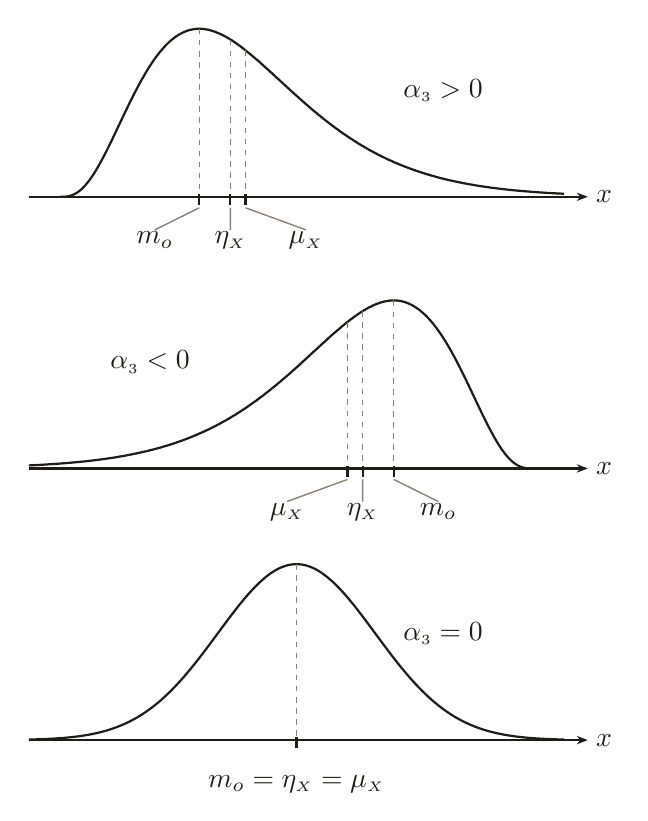
\begin{tikzpicture}[
  x=1cm,
  y=5.6cm,
  every node/.style={font=\normalsize, journalink},
  axis/.style={journalink, line width=0.8pt, -{Stealth[length=4pt]}},
  tick/.style={journalink, line width=0.8pt},
  curve/.style={journalink, line width=0.8pt},
  guide/.style={journalmuted, line width=0.5pt, dash pattern=on 2pt off 2pt},
  leader/.style={journalmuted, line width=0.5pt}
]

% =====================================================================
% top panel: Gamma(4, 1.7), alpha_3 = 1
% =====================================================================
\begin{scope}[yshift=0cm]
  \draw[curve] plot[domain=0:6.4, samples=300, smooth] (\x,{\gammafour{\x}});
  \draw[axis] (-0.4,0) -- (6.7,0);
  \node[anchor=west, inner sep=2.8pt] at (6.7,0) {$x$};

  \draw[guide] (1.764706,0.380871) -- (1.764706,0);
  \draw[guide] (2.160036,0.356674) -- (2.160036,0);
  \draw[guide] (2.352941,0.332124) -- (2.352941,0);
  \foreach \p in {1.764706, 2.160036, 2.352941}
    \draw[tick] ([yshift=0.035cm]\p,0) -- ([yshift=-0.106cm]\p,0);

  \draw[leader] ([yshift=-0.14cm]1.764706,0) -- ([yshift=-0.42cm]1.20,0);
  \draw[leader] ([yshift=-0.14cm]2.160036,0) -- ([yshift=-0.42cm]2.16,0);
  \draw[leader] ([yshift=-0.14cm]2.352941,0) -- ([yshift=-0.42cm]3.12,0);
  \node[anchor=north, inner sep=0pt] at ([yshift=-0.44cm]1.20,0) {$m_{o}$};
  \node[anchor=north, inner sep=0pt] at ([yshift=-0.44cm]2.16,0)
    {$\eta_{\sssig X}$};
  \node[anchor=north, inner sep=0pt] at ([yshift=-0.44cm]3.12,0)
    {$\mu_{\sssig X}$};

  \node[anchor=west, inner sep=0pt] at ([yshift=1.35cm]4.35,0)
    {$\alpha_{\sssig 3}>0$};
\end{scope}

% =====================================================================
% middle panel: the same density mirrored in x = 3, alpha_3 = -1
% =====================================================================
\begin{scope}[yshift=-3.45cm]
  \draw[curve] plot[domain=-0.4:6, samples=300, smooth]
    (\x,{\gammafour{6-\x}});
  \draw[axis] (-0.4,0) -- (6.7,0);
  \node[anchor=west, inner sep=2.8pt] at (6.7,0) {$x$};

  \draw[guide] (3.647059,0.332124) -- (3.647059,0);
  \draw[guide] (3.839964,0.356674) -- (3.839964,0);
  \draw[guide] (4.235294,0.380871) -- (4.235294,0);
  \foreach \p in {3.647059, 3.839964, 4.235294}
    \draw[tick] ([yshift=0.035cm]\p,0) -- ([yshift=-0.106cm]\p,0);

  \draw[leader] ([yshift=-0.14cm]3.647059,0) -- ([yshift=-0.42cm]2.88,0);
  \draw[leader] ([yshift=-0.14cm]3.839964,0) -- ([yshift=-0.42cm]3.84,0);
  \draw[leader] ([yshift=-0.14cm]4.235294,0) -- ([yshift=-0.42cm]4.80,0);
  \node[anchor=north, inner sep=0pt] at ([yshift=-0.44cm]2.88,0)
    {$\mu_{\sssig X}$};
  \node[anchor=north, inner sep=0pt] at ([yshift=-0.44cm]3.84,0)
    {$\eta_{\sssig X}$};
  \node[anchor=north, inner sep=0pt] at ([yshift=-0.44cm]4.80,0) {$m_{o}$};

  \node[anchor=east, inner sep=0pt] at ([yshift=1.35cm]1.65,0)
    {$\alpha_{\sssig 3}<0$};
\end{scope}

% =====================================================================
% bottom panel: N(3, 1), alpha_3 = 0
% =====================================================================
\begin{scope}[yshift=-6.90cm]
  \draw[curve] plot[domain=-0.4:6.4, samples=300, smooth]
    (\x,{0.3989423*exp(-(\x-3)*(\x-3)/2)});
  \draw[axis] (-0.4,0) -- (6.7,0);
  \node[anchor=west, inner sep=2.8pt] at (6.7,0) {$x$};

  \draw[guide] (3,0.398942) -- (3,0);
  \draw[tick] ([yshift=0.035cm]3,0) -- ([yshift=-0.106cm]3,0);
  \node[anchor=north, inner sep=0pt] at ([yshift=-0.44cm]3,0)
    {$m_{o}=\eta_{\sssig X}=\mu_{\sssig X}$};

  \node[anchor=west, inner sep=0pt] at ([yshift=1.35cm]4.35,0)
    {$\alpha_{\sssig 3}=0$};
\end{scope}

\end{tikzpicture}
\end{document}
